%!TEX root = ../book.tex

% ******************************* Part: Relational Databases ****************************

%this is a overarching PART that can be replicated to change overarching areas in the book
\part{Relational Databases}
\label{part:relationaldatabases}
This \lcnamecref{part:relationaldatabases} area allows me to write something about the PART.

% ******************************* Chapter: Introduction ****************************
\chapter{Introduction}
\label{chap:relational:introduction}
This part of the book teaches the basics of relational databases. It will walk you through the basics of relational databases, and how to design a database from scratch. After this, it will teach you how to create ER and EER diagrams, and how to design a database from an ER model. Finally, it will teach you how to normalize a database to the 4th normal form.


\section{What exactly is a relational database?}

\section{Why use a relational database?}

\section{What is SQL?}

\section{What is PostgreSQL?}

\section{Getting to terms with the terminology}
\begin{figure}[h]
    \centering
    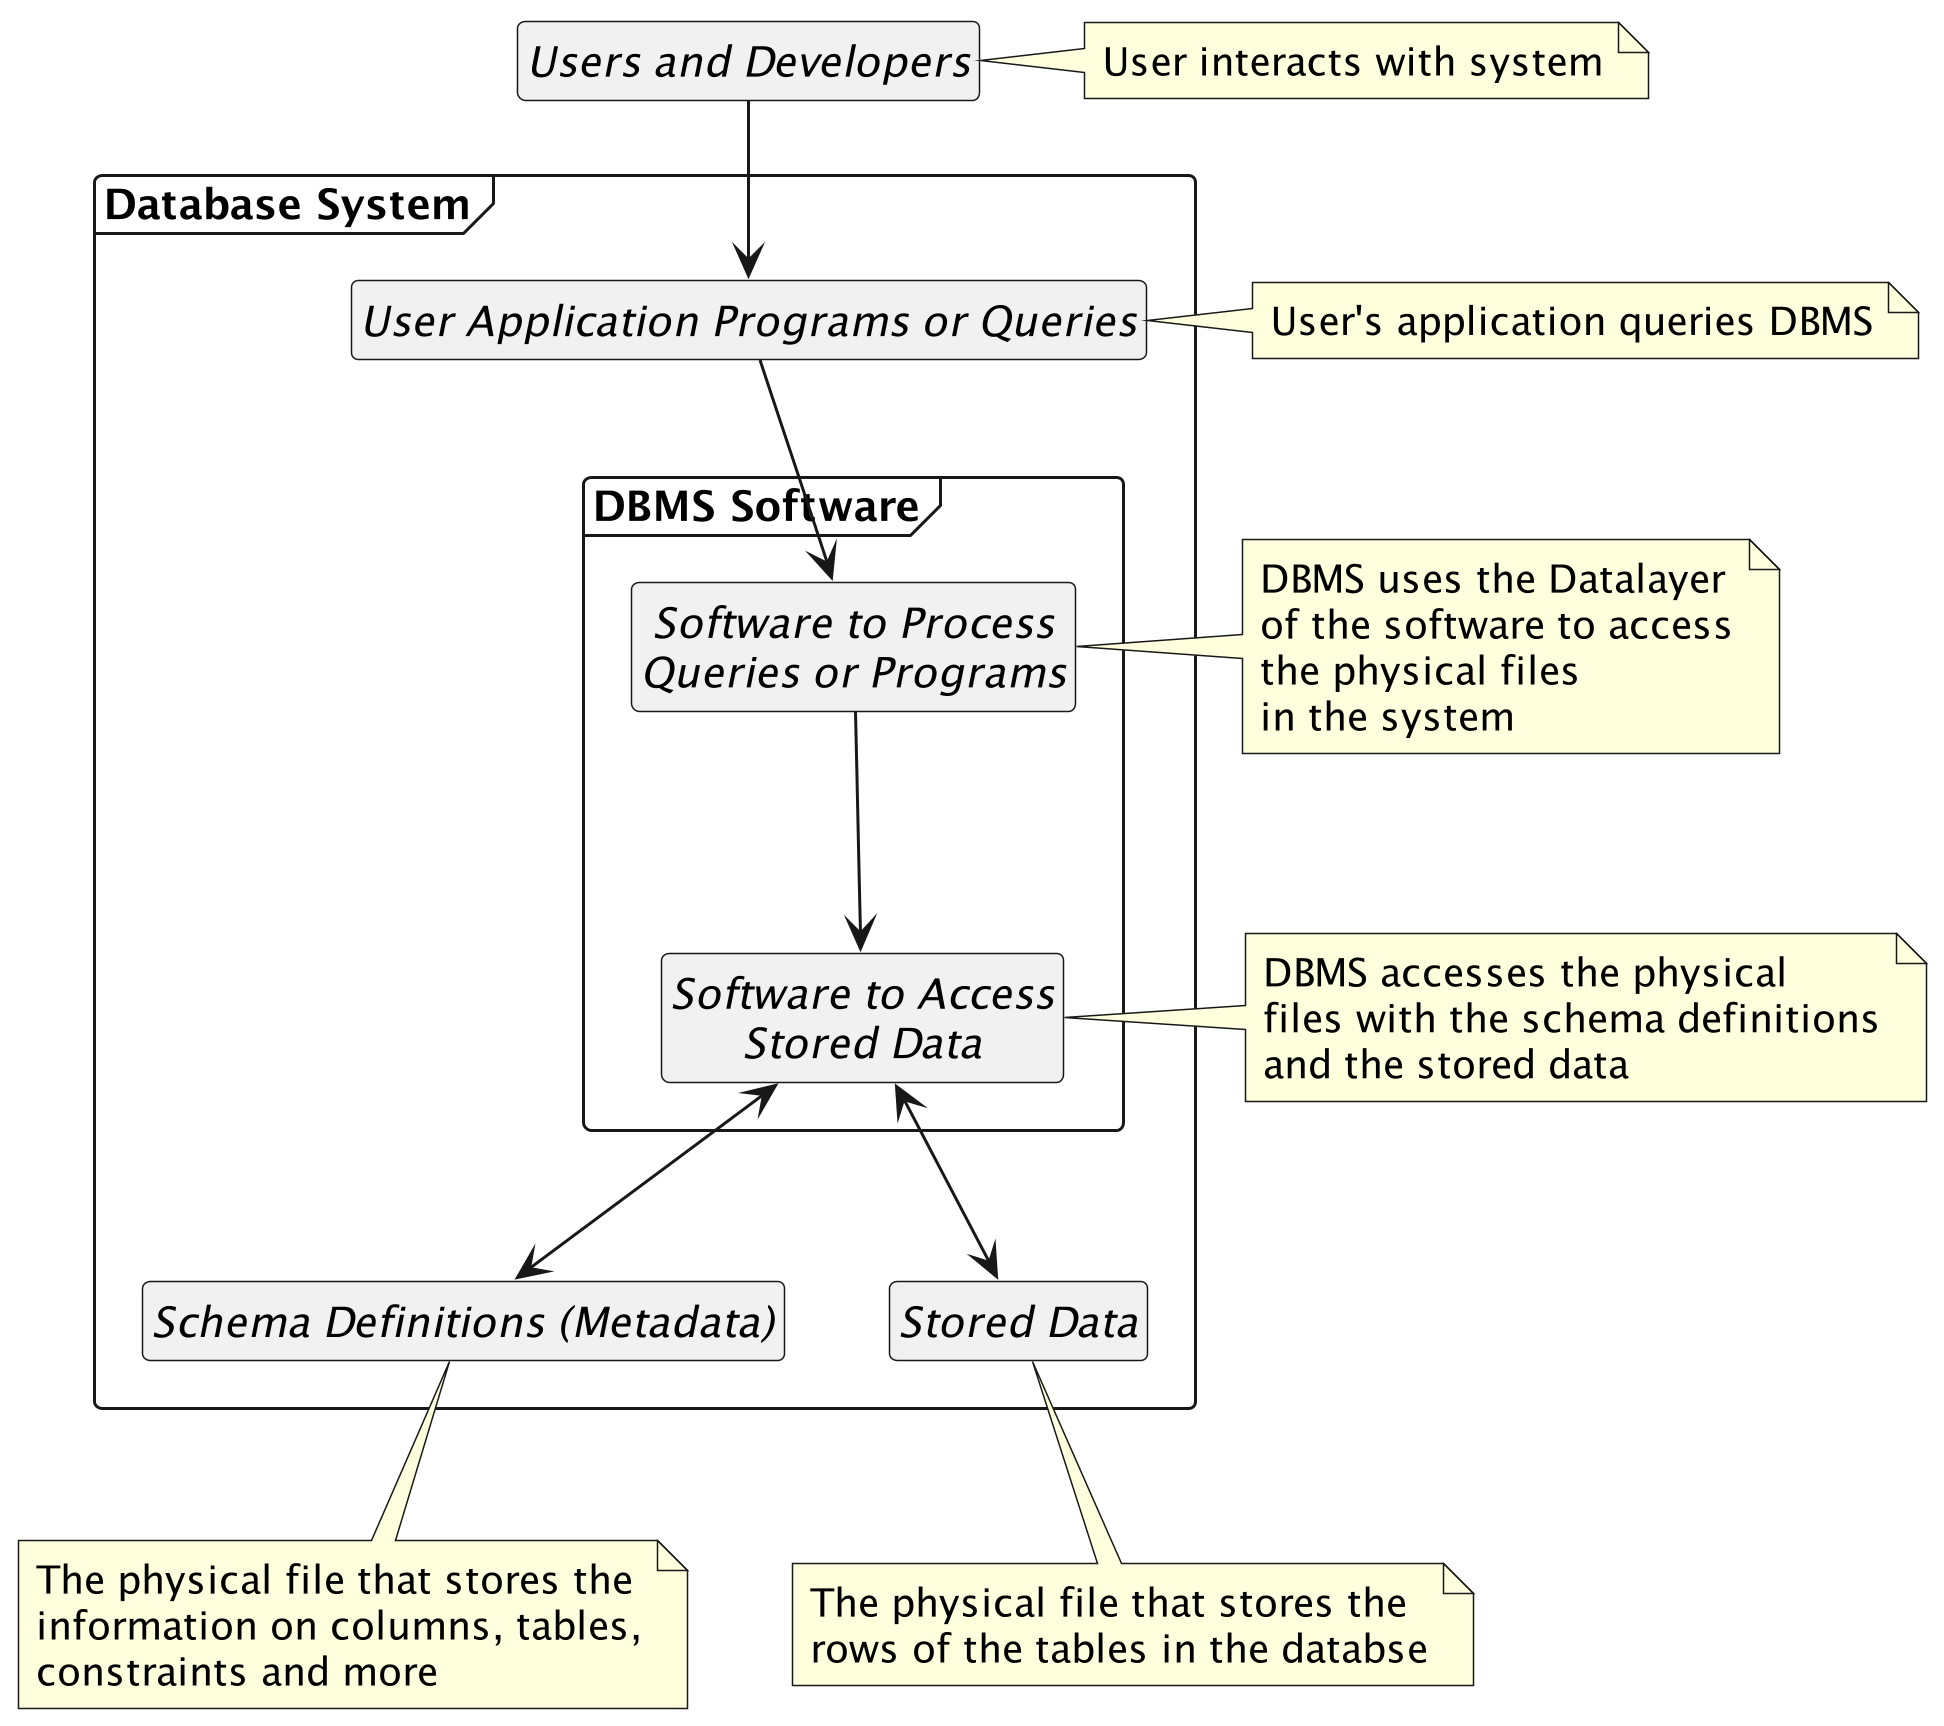
\includegraphics[width=1\textwidth]{content/1-relational-databases/figures/1.dbms-definitions.png}
    \caption{High Level Explanation of a Database Management System}
    \label{fig:1.dbms-definitions.png}
\end{figure}

\begin{figure}[h]
    \centering
    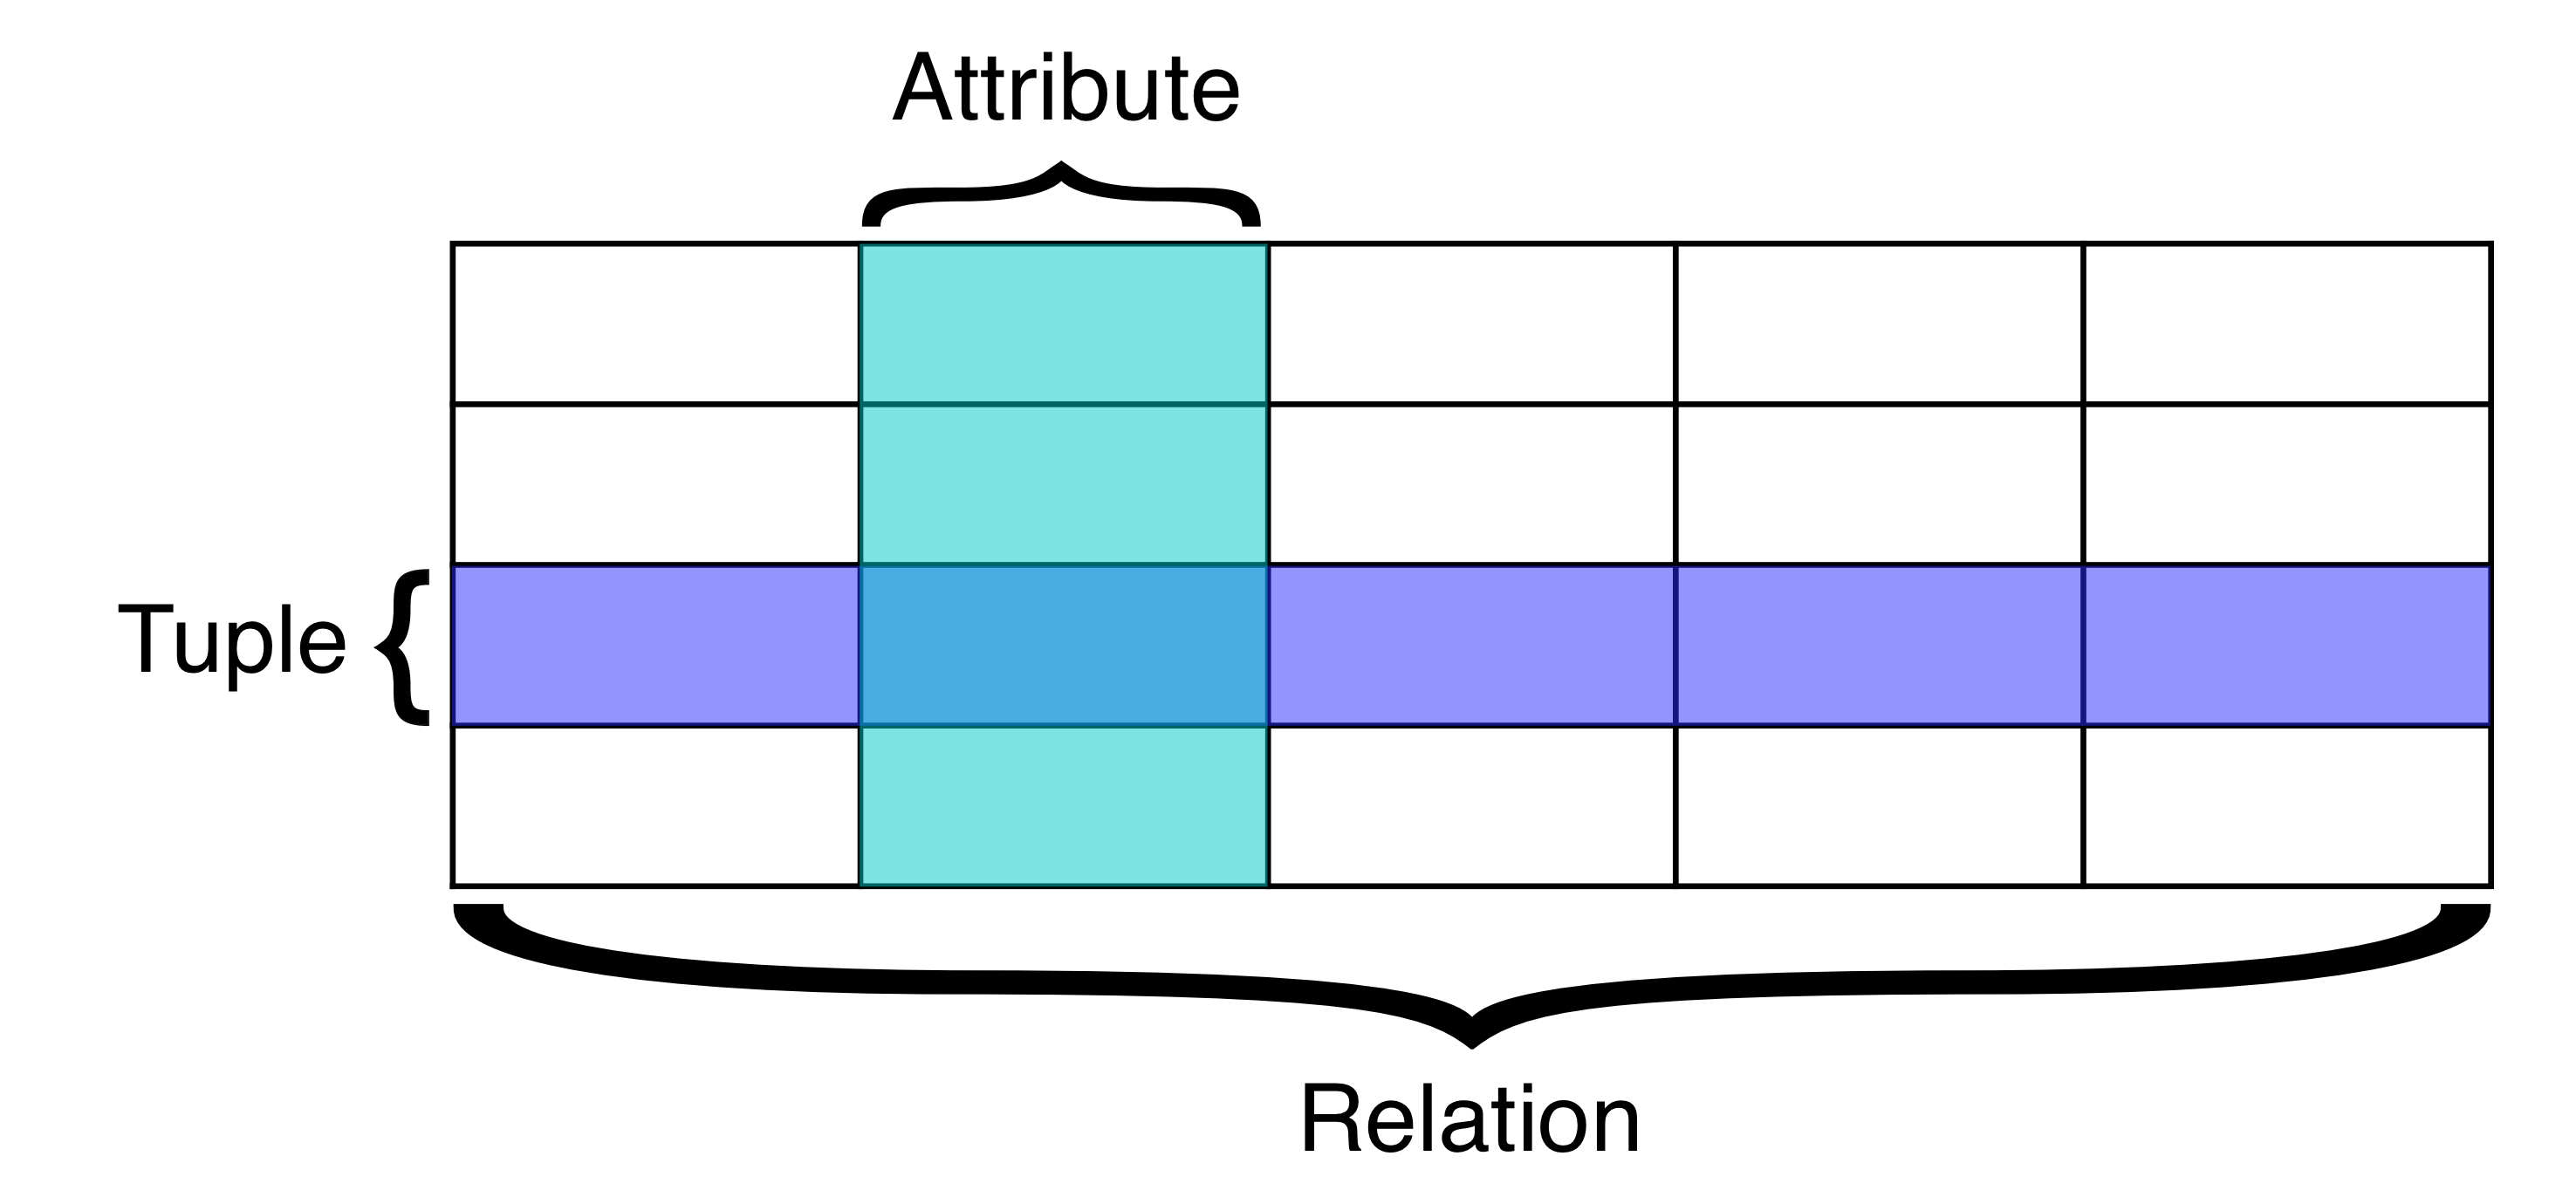
\includegraphics[width=1\textwidth]{content/1-relational-databases/figures/2.table-definitions.png}
    \caption{Table Terminology (Artist: Chris Martin)}
    \label{fig:2.table-definitions.png}
\end{figure}

\section{Getting Started}


% ******************************* Chapter: Relational Database Basics ****************************
\chapter{Relational Database Basics}
\label{chap:relational:relational-database-basics}
This chapter contains the basic building blocks to get started with basic relational databases.

\section{Creating your first database}

\section{Managing Databases}

\subsection{Creating a database}
\begin{minted}[fontsize=\footnotesize]{postgresql}
    -- Creating a database with full syntax
    CREATE DATABASE database_name
    WITH
        [OWNER =  role_name]
        [TEMPLATE = template]
        [ENCODING = encoding]
        [LC_COLLATE = collate]
        [LC_CTYPE = ctype]
        [TABLESPACE = tablespace_name]
        [ALLOW_CONNECTIONS = true | false]
        [CONNECTION LIMIT = max_concurrent_connection]
        [IS_TEMPLATE = true | false ]
\end{minted}

\begin{minted}[fontsize=\footnotesize]{postgresql}
    -- Creating an ACME database with minimal syntax
    CREATE DATABASE Acme;
\end{minted}

\begin{minted}[fontsize=\footnotesize]{postgresql}
    -- Creating a ACME database with enabled options
    CREATE DATABASE Acme 
    WITH
        OWNER = postgres
        CONNECTION LIMIT = 50;
        IS_TEMPLATE = false;
\end{minted}

\subsection{Altering a database}
\begin{minted}[fontsize=\footnotesize]{postgresql}
    -- Create a table
    CREATE TABLE tableName (
        tableName_id SERIAL PRIMARY KEY, -- auto incrementing id
        username VARCHAR (50) UNIQUE NOT NULL, -- unique username
        password VARCHAR (250) NOT NULL -- never store in plain text
    );
\end{minted}

\subsection{Deleting a database}
\begin{minted}[fontsize=\footnotesize]{postgresql}
    -- Create a table
    CREATE TABLE tableName (
        tableName_id SERIAL PRIMARY KEY, -- auto incrementing id
        username VARCHAR (50) UNIQUE NOT NULL, -- unique username
        password VARCHAR (250) NOT NULL -- never store in plain text
    );
\end{minted}

\subsection{Switch databases}
\begin{minted}[fontsize=\footnotesize]{sql}
    /* Change to database_name
     * This does not work with PostgreSQL */
    USE database_name;
\end{minted}

\begin{minted}[fontsize=\footnotesize]{psql}
    -- Change to database_name from psql command line
    \connect database_name
\end{minted}


\section{Managing Tables}

\subsection{Creating tables}
\begin{minted}[fontsize=\footnotesize]{postgresql}
    -- Create a table
    CREATE TABLE tableName (
        tableName_id SERIAL PRIMARY KEY, -- auto incrementing id
        username VARCHAR (50) UNIQUE NOT NULL, -- unique username
        password VARCHAR (250) NOT NULL -- never store in plain text
    );
\end{minted}

\begin{minted}[fontsize=\footnotesize]{postgresql}
    -- Create account table
    CREATE TABLE account (
        id serial PRIMARY KEY,
        username VARCHAR (50) UNIQUE NOT NULL,
        created_on TIMESTAMP NOT NULL, 
        last_login TIMESTAMP
    );
    
    /* Create blog entries table
     * the created_by column references the 
     * id column in the account table */
    CREATE TABLE blog_entries (
        id serial PRIMARY KEY, 
        header VARCHAR (255) NOT NULL,
        body TEXT NOT NULL,
        created_by INTEGER NOT NULL REFERENCES account (id)
    );
\end{minted}

\subsection{Altering tables}
\begin{minted}[fontsize=\footnotesize]{postgresql}
    -- Create a table
    CREATE TABLE account (
        user_id SERIAL PRIMARY KEY,
        username VARCHAR (50) UNIQUE NOT NULL,
        password VARCHAR (50) NOT NULL,
        email VARCHAR (355) UNIQUE NOT NULL,
        created_on TIMESTAMP NOT NULL,
        last_login TIMESTAMP
    );
\end{minted}

\subsection{Deleting tables}
\begin{minted}[fontsize=\footnotesize]{postgresql}
    -- Create a table
    CREATE TABLE account (
        user_id SERIAL PRIMARY KEY,
        username VARCHAR (50) UNIQUE NOT NULL,
        password VARCHAR (50) NOT NULL,
        email VARCHAR (355) UNIQUE NOT NULL,
        created_on TIMESTAMP NOT NULL,
        last_login TIMESTAMP
    );
\end{minted}

\section{CRUD Operations}

\section{Joins and querying related tables}

% ******************************* Chapter: ER, EER Modeling and Database Design ****************************
\chapter{ER, EER Modeling and Database Design}
\label{chap:relational:eer-modeling-and-database-design}
This chapter teaches basic ER and ER modelling, and how to design a database from an ER model.

\section{The purpose of ER and EER modeling}
\section{Diagram Elements}
\section{ER versus EER modeling}
\section{Mapping to tables}

% ******************************* Chapter: Database Normalization ****************************
\chapter{Database Normalization}
\label{chap:relational:database-normalization}
This chapter teaches database normalization to the 4th normal form.

\section{What is database normalization?}
\section{Shorthand techniques}
\section{First normal form}
\section{Second normal form}
\section{Third normal form}
\section{Fourth normal form}
\section{Normalization of other formats}

% ******************************* Chapter: Advanced Relational Databases ****************************
\chapter{Advanced Relational Databases}
\label{chap:relational:advanced-relational-databases}
This chapter teaches advanced relational database concepts.

\section{Transactions}
\section{Indexes}
\section{Views}
\section{Stored Procedures}
\section{Triggers}
\section{User Defined Functions}
\section{Security}
\section{Performance Tuning}


